\documentclass[]{article}
\usepackage{hyperref}
\usepackage[a4paper, total={6in, 8in}]{geometry}
\usepackage{caption}
\usepackage{algpseudocodex}
\usepackage{algorithm}
\usepackage{amsmath}
\usepackage{listings}
\usepackage{graphicx}
\usepackage{setspace}
\usepackage{subfiles}
\usepackage{xcolor}
\usepackage{enumerate}
\usepackage{tabularray}
\usepackage{array}
\usepackage{xepersian}
\settextfont{XB Niloofar}

% \setlength{\columnseprule}{0.4pt}

\begin{document}
سه فرآیند
\lr{P3, P2, P1}
با زمان اجرا و زمان ورود زیر را در نظر بگیرید و به موارد خواسته شده پاسخ دهید.
(عدد بالاتر بیانگر اولویت بالاتر است.)
\begin{table}[H]
      \centering
      \begin{tblr}{|c|c|c|c|}
            \hline
            زمان اجرا & زمان ورود & اولویت & فرآیند \\ \hline
            4         & $t$       & 2      & $P1$   \\ \hline
            2         & $t$       & 0      & $P2$   \\ \hline
            1         & $t+3$     & 1      & $P3$   \\
            \hline
      \end{tblr}
\end{table}

\begin{enumerate}[(A)]
      \item متوسط زمان پاسخگویی با روش SJF
            \begin{table}[H]
                  \centering
                  \begin{tblr}{ l l }
                        \begin{tblr}{l l}
                              $wT(P_1) = t + 2 - t = 2$
                               & $T(P_1) = 2 + 4 = 6$
                              \\
                              $wT(P_2) = t - t = 0$
                               & $T(P_2) = 0 + 2 = 2$
                              \\
                              $wT(P_3) = t + 6 - (t+3) = 3$
                               & $T(P_3) = 3 + 1 = 4$
                        \end{tblr}
                         & \begin{tblr}{c}
                                 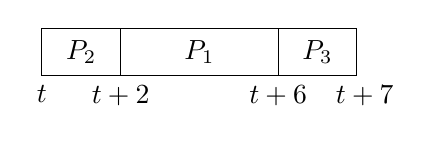
\begin{tikzpicture}
                                    % Draw the main rectangle
                                    \draw (0,0) rectangle (1,0.6) node[midway] {$P_2$};
                                    \draw (1,0) rectangle (3,0.6) node[midway] {$P_1$};
                                    \draw (3,0) rectangle (4,0.6) node[midway] {$P_3$};

                                    % Draw time labels
                                    \node[below] at (0,0) {$t$};
                                    \node[below] at (1,0) {$t+2$};
                                    \node[below] at (3,0) {$t+6$};
                                    \node[below] at (4.1,0) {$t+7$};
                              \end{tikzpicture}
                                  & \\
                                 $AvgT = \dfrac{6+2+4}{3} = 4$
                           \end{tblr}
                  \end{tblr}
            \end{table}
      \item متوسط زمان پاسخگویی با روش FIFO
            \begin{table}[H]
                  \centering
                  \begin{tblr}{ l l }
                        \begin{tblr}{l l}
                              $wT(P_1) = t - t= 0$
                               & $T(P_1) = 0 + 4 = 4$
                              \\
                              $wT(P_2) = t+4-t = 4$
                               & $T(P_2) = 4 + 2 = 6$
                              \\
                              $wT(P_3) = t + 6 - (t+3) = 3$
                               & $T(P_3) = 3 + 1 = 4$
                        \end{tblr}
                         & \begin{tblr}{c}
                                 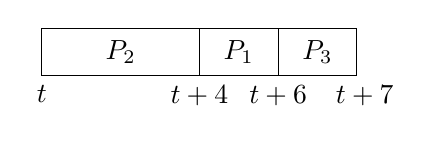
\begin{tikzpicture}
                                    % Draw the main rectangle
                                    \draw (0,0) rectangle (2,0.6) node[midway] {$P_2$};
                                    \draw (2,0) rectangle (3,0.6) node[midway] {$P_1$};
                                    \draw (3,0) rectangle (4,0.6) node[midway] {$P_3$};

                                    % Draw time labels
                                    \node[below] at (0,0) {$t$};
                                    \node[below] at (2,0) {$t+4$};
                                    \node[below] at (3,0) {$t+6$};
                                    \node[below] at (4.1,0) {$t+7$};
                              \end{tikzpicture}
                                  & \\
                                 $AvgT = \dfrac{4+6+4}{3} = \dfrac{14}{3}$
                           \end{tblr}
                  \end{tblr}
            \end{table}
      \item متوسط زمان پاسخگویی با روش SRT
            \begin{table}[H]
                  \centering
                  \begin{tblr}{ l l }
                        \begin{tblr}{l l}
                              $wT(P_1) = (t+2) - t +$ \\ $ t + 4 - (t+3)= 3$
                               & $T(P_1) = 3 + 4 = 7$
                              \\
                              $wT(P_2) = t-t = 0$
                               & $T(P_2) = 0 + 2 = 2$
                              \\
                              $wT(P_3) = t - t = 0$
                               & $T(P_3) = 0 + 1 = 1$
                        \end{tblr}
                         & \begin{tblr}{c}
                                 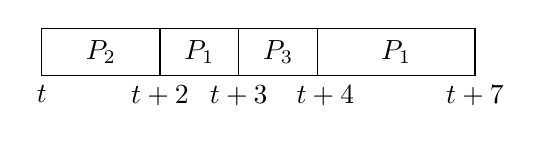
\begin{tikzpicture}
                                    % Draw the main rectangle
                                    \draw (0,0) rectangle (1.5,0.6) node[midway] {$P_2$};
                                    \draw (1.5,0) rectangle (2.5,0.6) node[midway] {$P_1$};
                                    \draw (2.5,0) rectangle (3.5,0.6) node[midway] {$P_3$};
                                    \draw (3.5,0) rectangle (5.5,0.6) node[midway] {$P_1$};

                                    % Draw time labels
                                    \node[below] at (0,0) {$t$};
                                    \node[below] at (1.5,0) {$t+2$};
                                    \node[below] at (2.5,0) {$t+3$};
                                    \node[below] at (3.6,0) {$t+4$};
                                    \node[below] at (5.5,0) {$t+7$};
                              \end{tikzpicture}
                                  & \\
                                 $AvgT = \dfrac{7+2+1}{3} = \dfrac{10}{3}$
                           \end{tblr}
                  \end{tblr}
            \end{table}
      \item متوسط زمان پاسخگویی با روش اولویت
            \begin{table}[H]
                  \centering
                  \begin{tblr}{ l l }
                        \begin{tblr}{l l}
                              $wT(P_1) = t - t= 0$
                               & $T(P_1) = 0 + 4 = 4$
                              \\
                              $wT(P_2) = t+5-t = 5$
                               & $T(P_2) = 5 + 2 = 7$
                              \\
                              $wT(P_3) = t + 4 - (t+3) = 1$
                               & $T(P_3) = 1 + 1 = 2$
                        \end{tblr}
                         & \begin{tblr}{c}
                                 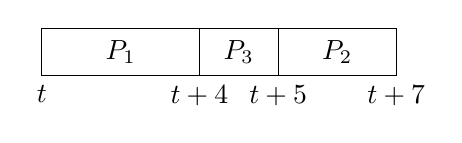
\begin{tikzpicture}
                                    % Draw the main rectangle
                                    \draw (0,0) rectangle (2,0.6) node[midway] {$P_1$};
                                    \draw (2,0) rectangle (3,0.6) node[midway] {$P_3$};
                                    \draw (3,0) rectangle (4.5,0.6) node[midway] {$P_2$};

                                    % Draw time labels
                                    \node[below] at (0,0) {$t$};
                                    \node[below] at (2,0) {$t+4$};
                                    \node[below] at (3,0) {$t+5$};
                                    \node[below] at (4.5,0) {$t+7$};
                              \end{tikzpicture}
                                  & \\
                                 $AvgT = \dfrac{4+7+2}{3} = \dfrac{13}{3}$
                           \end{tblr}
                  \end{tblr}
            \end{table}
\end{enumerate}

\end{document}